

%% bare_jrnl.tex
%% V1.4
%% 2012/12/27
%% by Michael Shell
%% see http://www.michaelshell.org/
%% for current contact information.
%%
%% This is a skeleton file demonstrating the use of IEEEtran.cls
%% (requires IEEEtran.cls version 1.8 or later) with an IEEE journal paper.
%%
%% Support sites:
%% http://www.michaelshell.org/tex/ieeetran/
%% http://www.ctan.org/tex-archive/macros/latex/contrib/IEEEtran/
%% and
%% http://www.ieee.org/



% *** Authors should verify (and, if needed, correct) their LaTeX system  ***
% *** with the testflow diagnostic prior to trusting their LaTeX platform ***
% *** with production work. IEEE's font choices can trigger bugs that do  ***
% *** not appear when using other class files.                            ***
% The testflow support page is at:
% http://www.michaelshell.org/tex/testflow/


%%*************************************************************************
%% Legal Notice:
%% This code is offered as-is without any warranty either expressed or
%% implied; without even the implied warranty of MERCHANTABILITY or
%% FITNESS FOR A PARTICULAR PURPOSE! 
%% User assumes all risk.
%% In no event shall IEEE or any contributor to this code be liable for
%% any damages or losses, including, but not limited to, incidental,
%% consequential, or any other damages, resulting from the use or misuse
%% of any information contained here.
%%
%% All comments are the opinions of their respective authors and are not
%% necessarily endorsed by the IEEE.
%%
%% This work is distributed under the LaTeX Project Public License (LPPL)
%% ( http://www.latex-project.org/ ) version 1.3, and may be freely used,
%% distributed and modified. A copy of the LPPL, version 1.3, is included
%% in the base LaTeX documentation of all distributions of LaTeX released
%% 2003/12/01 or later.
%% Retain all contribution notices and credits.
%% ** Modified files should be clearly indicated as such, including  **
%% ** renaming them and changing author support contact information. **
%%
%% File list of work: IEEEtran.cls, IEEEtran_HOWTO.pdf, bare_adv.tex,
%%                    bare_conf.tex, bare_jrnl.tex, bare_jrnl_compsoc.tex,
%%                    bare_jrnl_transmag.tex
%%*************************************************************************

% Note that the a4paper option is mainly intended so that authors in
% countries using A4 can easily print to A4 and see how their papers will
% look in print - the typesetting of the document will not typically be
% affected with changes in paper size (but the bottom and side margins will).
% Use the testflow package mentioned above to verify correct handling of
% both paper sizes by the user's LaTeX system.
%
% Also note that the "draftcls" or "draftclsnofoot", not "draft", option
% should be used if it is desired that the figures are to be displayed in
% draft mode.
%
\documentclass[journal]{IEEEtran}
%
% If IEEEtran.cls has not been installed into the LaTeX system files,
% manually specify the path to it like:
% \documentclass[journal]{../sty/IEEEtran}


% Some very useful LaTeX packages include:
% (uncomment the ones you want to load)


% *** MISC UTILITY PACKAGES ***
%
%\usepackage{ifpdf}
% Heiko Oberdiek's ifpdf.sty is very useful if you need conditional
% compilation based on whether the output is pdf or dvi.
% usage:
% \ifpdf
%   % pdf code
% \else
%   % dvi code
% \fi
% The latest version of ifpdf.sty can be obtained from:
% http://www.ctan.org/tex-archive/macros/latex/contrib/oberdiek/
% Also, note that IEEEtran.cls V1.7 and later provides a builtin
% \ifCLASSINFOpdf conditional that works the same way.
% When switching from latex to pdflatex and vice-versa, the compiler may
% have to be run twice to clear warning/error messages.

% *** CITATION PACKAGES ***
%
\usepackage{cite}
% cite.sty was written by Donald Arseneau
% V1.6 and later of IEEEtran pre-defines the format of the cite.sty package
% \cite{} output to follow that of IEEE. Loading the cite package will
% result in citation numbers being automatically sorted and properly
% "compressed/ranged". e.g., [1], [9], [2], [7], [5], [6] without using
% cite.sty will become [1], [2], [5]--[7], [9] using cite.sty. cite.sty's
% \cite will automatically add leading space, if needed. Use cite.sty's
% noadjust option (cite.sty V3.8 and later) if you want to turn this off
% such as if a citation ever needs to be enclosed in parenthesis.
% cite.sty is already installed on most LaTeX systems. Be sure and use
% version 4.0 (2003-05-27) and later if using hyperref.sty. cite.sty does
% not currently provide for hyperlinked citations.
% The latest version can be obtained at:
% http://www.ctan.org/tex-archive/macros/latex/contrib/cite/
% The documentation is contained in the cite.sty file itself.




% *** GRAPHICS RELATED PACKAGES ***
%
\ifCLASSINFOpdf
   \usepackage[pdftex]{graphicx}
  % declare the path(s) where your graphic files are
   \graphicspath{{./graphics/}}%{../jpeg/}}
  % and their extensions so you won't have to specify these with
  % every instance of \includegraphics
   \DeclareGraphicsExtensions{.pdf,.jpeg,.png}
\else
  % or other class option (dvipsone, dvipdf, if not using dvips). graphicx
  % will default to the driver specified in the system graphics.cfg if no
  % driver is specified.
  % \usepackage[dvips]{graphicx}
  % declare the path(s) where your graphic files are
  % \graphicspath{{../eps/}}
  % and their extensions so you won't have to specify these with
  % every instance of \includegraphics
  % \DeclareGraphicsExtensions{.eps}
\fi
% graphicx was written by David Carlisle and Sebastian Rahtz. It is
% required if you want graphics, photos, etc. graphicx.sty is already
% installed on most LaTeX systems. The latest version and documentation
% can be obtained at: 
% http://www.ctan.org/tex-archive/macros/latex/required/graphics/
% Another good source of documentation is "Using Imported Graphics in
% LaTeX2e" by Keith Reckdahl which can be found at:
% http://www.ctan.org/tex-archive/info/epslatex/
%
% latex, and pdflatex in dvi mode, support graphics in encapsulated
% postscript (.eps) format. pdflatex in pdf mode supports graphics
% in .pdf, .jpeg, .png and .mps (metapost) formats. Users should ensure
% that all non-photo figures use a vector format (.eps, .pdf, .mps) and
% not a bitmapped formats (.jpeg, .png). IEEE frowns on bitmapped formats
% which can result in "jaggedy"/blurry rendering of lines and letters as
% well as large increases in file sizes.
%
% You can find documentation about the pdfTeX application at:
% http://www.tug.org/applications/pdftex





% *** MATH PACKAGES ***
%
\usepackage[cmex10]{amsmath}
% A popular package from the American Mathematical Society that provides
% many useful and powerful commands for dealing with mathematics. If using
% it, be sure to load this package with the cmex10 option to ensure that
% only type 1 fonts will utilized at all point sizes. Without this option,
% it is possible that some math symbols, particularly those within
% footnotes, will be rendered in bitmap form which will result in a
% document that can not be IEEE Xplore compliant!
%
% Also, note that the amsmath package sets \interdisplaylinepenalty to 10000
% thus preventing page breaks from occurring within multiline equations. Use:
\interdisplaylinepenalty=2500
% after loading amsmath to restore such page breaks as IEEEtran.cls normally
% does. amsmath.sty is already installed on most LaTeX systems. The latest
% version and documentation can be obtained at:
% http://www.ctan.org/tex-archive/macros/latex/required/amslatex/math/





% *** SPECIALIZED LIST PACKAGES ***
%
\usepackage{otherstuff/algorithm}
\usepackage{otherstuff/algorithmic}
% algorithmic.sty was written by Peter Williams and Rogerio Brito.
% This package provides an algorithmic environment fo describing algorithms.
% You can use the algorithmic environment in-text or within a figure
% environment to provide for a floating algorithm. Do NOT use the algorithm
% floating environment provided by algorithm.sty (by the same authors) or
% algorithm2e.sty (by Christophe Fiorio) as IEEE does not use dedicated
% algorithm float types and packages that provide these will not provide
% correct IEEE style captions. The latest version and documentation of
% algorithmic.sty can be obtained at:
% http://www.ctan.org/tex-archive/macros/latex/contrib/algorithms/
% There is also a support site at:
% http://algorithms.berlios.de/index.html
% Also of interest may be the (relatively newer and more customizable)
% algorithmicx.sty package by Szasz Janos:
% http://www.ctan.org/tex-archive/macros/latex/contrib/algorithmicx/




% *** ALIGNMENT PACKAGES ***
%
\usepackage{array}
% Frank Mittelbach's and David Carlisle's array.sty patches and improves
% the standard LaTeX2e array and tabular environments to provide better
% appearance and additional user controls. As the default LaTeX2e table
% generation code is lacking to the point of almost being broken with
% respect to the quality of the end results, all users are strongly
% advised to use an enhanced (at the very least that provided by array.sty)
% set of table tools. array.sty is already installed on most systems. The
% latest version and documentation can be obtained at:
% http://www.ctan.org/tex-archive/macros/latex/required/tools/


% IEEEtran contains the IEEEeqnarray family of commands that can be used to
% generate multiline equations as well as matrices, tables, etc., of high
% quality.




% *** SUBFIGURE PACKAGES ***
%\ifCLASSOPTIONcompsoc
%  \usepackage[caption=false,font=normalsize,labelfont=sf,textfont=sf]{subfig}
%\else
%  \usepackage[caption=false,font=footnotesize]{subfig}
%\fi
% subfig.sty, written by Steven Douglas Cochran, is the modern replacement
% for subfigure.sty, the latter of which is no longer maintained and is
% incompatible with some LaTeX packages including fixltx2e. However,
% subfig.sty requires and automatically loads Axel Sommerfeldt's caption.sty
% which will override IEEEtran.cls' handling of captions and this will result
% in non-IEEE style figure/table captions. To prevent this problem, be sure
% and invoke subfig.sty's "caption=false" package option (available since
% subfig.sty version 1.3, 2005/06/28) as this is will preserve IEEEtran.cls
% handling of captions.
% Note that the Computer Society format requires a larger sans serif font
% than the serif footnote size font used in traditional IEEE formatting
% and thus the need to invoke different subfig.sty package options depending
% on whether compsoc mode has been enabled.
%
% The latest version and documentation of subfig.sty can be obtained at:
% http://www.ctan.org/tex-archive/macros/latex/contrib/subfig/




% *** FLOAT PACKAGES ***
%
%\usepackage{fixltx2e}
% fixltx2e, the successor to the earlier fix2col.sty, was written by
% Frank Mittelbach and David Carlisle. This package corrects a few problems
% in the LaTeX2e kernel, the most notable of which is that in current
% LaTeX2e releases, the ordering of single and double column floats is not
% guaranteed to be preserved. Thus, an unpatched LaTeX2e can allow a
% single column figure to be placed prior to an earlier double column
% figure. The latest version and documentation can be found at:
% http://www.ctan.org/tex-archive/macros/latex/base/


%\usepackage{stfloats}
% stfloats.sty was written by Sigitas Tolusis. This package gives LaTeX2e
% the ability to do double column floats at the bottom of the page as well
% as the top. (e.g., "\begin{figure*}[!b]" is not normally possible in
% LaTeX2e). It also provides a command:
%\fnbelowfloat
% to enable the placement of footnotes below bottom floats (the standard
% LaTeX2e kernel puts them above bottom floats). This is an invasive package
% which rewrites many portions of the LaTeX2e float routines. It may not work
% with other packages that modify the LaTeX2e float routines. The latest
% version and documentation can be obtained at:
% http://www.ctan.org/tex-archive/macros/latex/contrib/sttools/
% Do not use the stfloats baselinefloat ability as IEEE does not allow
% \baselineskip to stretch. Authors submitting work to the IEEE should note
% that IEEE rarely uses double column equations and that authors should try
% to avoid such use. Do not be tempted to use the cuted.sty or midfloat.sty
% packages (also by Sigitas Tolusis) as IEEE does not format its papers in
% such ways.
% Do not attempt to use stfloats with fixltx2e as they are incompatible.
% Instead, use Morten Hogholm'a dblfloatfix which combines the features
% of both fixltx2e and stfloats:
%
% \usepackage{dblfloatfix}
% The latest version can be found at:
% http://www.ctan.org/tex-archive/macros/latex/contrib/dblfloatfix/




%\ifCLASSOPTIONcaptionsoff
%  \usepackage[nomarkers]{endfloat}
% \let\MYoriglatexcaption\caption
% \renewcommand{\caption}[2][\relax]{\MYoriglatexcaption[#2]{#2}}
%\fi
% endfloat.sty was written by James Darrell McCauley, Jeff Goldberg and 
% Axel Sommerfeldt. This package may be useful when used in conjunction with 
% IEEEtran.cls'  captionsoff option. Some IEEE journals/societies require that
% submissions have lists of figures/tables at the end of the paper and that
% figures/tables without any captions are placed on a page by themselves at
% the end of the document. If needed, the draftcls IEEEtran class option or
% \CLASSINPUTbaselinestretch interface can be used to increase the line
% spacing as well. Be sure and use the nomarkers option of endfloat to
% prevent endfloat from "marking" where the figures would have been placed
% in the text. The two hack lines of code above are a slight modification of
% that suggested by in the endfloat docs (section 8.4.1) to ensure that
% the full captions always appear in the list of figures/tables - even if
% the user used the short optional argument of \caption[]{}.
% IEEE papers do not typically make use of \caption[]'s optional argument,
% so this should not be an issue. A similar trick can be used to disable
% captions of packages such as subfig.sty that lack options to turn off
% the subcaptions:
% For subfig.sty:
% \let\MYorigsubfloat\subfloat
% \renewcommand{\subfloat}[2][\relax]{\MYorigsubfloat[]{#2}}
% However, the above trick will not work if both optional arguments of
% the \subfloat command are used. Furthermore, there needs to be a
% description of each subfigure *somewhere* and endfloat does not add
% subfigure captions to its list of figures. Thus, the best approach is to
% avoid the use of subfigure captions (many IEEE journals avoid them anyway)
% and instead reference/explain all the subfigures within the main caption.
% The latest version of endfloat.sty and its documentation can obtained at:
% http://www.ctan.org/tex-archive/macros/latex/contrib/endfloat/
%
% The IEEEtran \ifCLASSOPTIONcaptionsoff conditional can also be used
% later in the document, say, to conditionally put the References on a 
% page by themselves.




% *** PDF, URL AND HYPERLINK PACKAGES ***
%
\usepackage{url}
% url.sty was written by Donald Arseneau. It provides better support for
% handling and breaking URLs. url.sty is already installed on most LaTeX
% systems. The latest version and documentation can be obtained at:
% http://www.ctan.org/tex-archive/macros/latex/contrib/url/
% Basically, \url{my_url_here}.




% *** Do not adjust lengths that control margins, column widths, etc. ***
% *** Do not use packages that alter fonts (such as pslatex).         ***
% There should be no need to do such things with IEEEtran.cls V1.6 and later.
% (Unless specifically asked to do so by the journal or conference you plan
% to submit to, of course. )


% correct bad hyphenation here
%\hyphenation{optical networks semiconductor}



\begin{document}
%
% paper title
% can use linebreaks \\ within to get better formatting as desired
% Do not put math or special symbols in the title.
\title{TDT4260 Project Report}
%
%
% author names and IEEE memberships
% note positions of commas and nonbreaking spaces ( ~ ) LaTeX will not break
% a structure at a ~ so this keeps an author's name from being broken across
% two lines.
% use \thanks{} to gain access to the first footnote area
% a separate \thanks must be used for each paragraph as LaTeX2e's \thanks
% was not built to handle multiple paragraphs
%

\author{Christopher~Benjamin~Westlye,
        Kaj~Palm,
        Raymond~Selvik,
       and~Trond~Einar~Snekvik}% <-this % stops a space
%\thanks{M. Shell is with the Department
%of Electrical and Computer Engineering, Georgia Institute of Technology, Atlanta,
%GA, 30332 USA e-mail: (see http://www.michaelshell.org/contact.html).}% <-this % stops a space
%\thanks{J. Doe and J. Doe are with Anonymous University.}% <-this % stops a space
%\thanks{Manuscript received April 19, 2005; revised December 27, 2012.}}

% note the % following the last \IEEEmembership and also \thanks - 
% these prevent an unwanted space from occurring between the last author name
% and the end of the author line. i.e., if you had this:
% 
% \author{....lastname \thanks{...} \thanks{...} }
%                     ^------------^------------^----Do not want these spaces!
%
% a space would be appended to the last name and could cause every name on that
% line to be shifted left slightly. This is one of those "LaTeX things". For
% instance, "\textbf{A} \textbf{B}" will typeset as "A B" not "AB". To get
% "AB" then you have to do: "\textbf{A}\textbf{B}"
% \thanks is no different in this regard, so shield the last } of each \thanks
% that ends a line with a % and do not let a space in before the next \thanks.
% Spaces after \IEEEmembership other than the last one are OK (and needed) as
% you are supposed to have spaces between the names. For what it is worth,
% this is a minor point as most people would not even notice if the said evil
% space somehow managed to creep in.



% The paper headers
%\markboth{Journal of \LaTeX\ Class Files,~Vol.~11, No.~4, December~2012}%
%{Shell \MakeLowercase{\textit{et al.}}: Bare Demo of IEEEtran.cls for Journals}

% The only time the second header will appear is for the odd numbered pages
% after the title page when using the twoside option.
% 
% *** Note that you probably will NOT want to include the author's ***
% *** name in the headers of peer review papers.                   ***
% You can use \ifCLASSOPTIONpeerreview for conditional compilation here if
% you desire.




% If you want to put a publisher's ID mark on the page you can do it like
% this:
%\IEEEpubid{0000--0000/00\$00.00~\copyright~2012 IEEE}
% Remember, if you use this you must call \IEEEpubidadjcol in the second
% column for its text to clear the IEEEpubid mark.



% use for special paper notices
%\IEEEspecialpapernotice{(Invited Paper)}




% make the title area
\maketitle

% As a general rule, do not put math, special symbols or citations
% in the abstract or keywords.
\begin{abstract}
This paper presents a pattern-recognizing prefetcher based on the DPT prefetching heuristic by Marius Grannae, Magnus Jahre and Lasse Natvig. The prefetcher attempts to achieve high accuracy through strict rules for the next fetch based on a previously recognized fetch sequence.
\end{abstract}

% Note that keywords are not normally used for peerreview papers.
%\begin{IEEEkeywords}
%IEEEtran, journal, \LaTeX, paper, template.
%\end{IEEEkeywords}



% For peer review papers, you can put extra information on the cover
% page as needed:
% \ifCLASSOPTIONpeerreview
% \begin{center} \bfseries EDICS Category: 3-BBND \end{center}
% \fi
%
% For peerreview papers, this IEEEtran command inserts a page break and
% creates the second title. It will be ignored for other modes.
\IEEEpeerreviewmaketitle


\section{Introduction}
% The very first letter is a 2 line initial drop letter followed
% by the rest of the first word in caps.
% 
% form to use if the first word consists of a single letter:
% \IEEEPARstart{A}{demo} file is ....
% 
% form to use if you need the single drop letter followed by
% normal text (unknown if ever used by IEEE):
% \IEEEPARstart{A}{}demo file is ....
% 
% Some journals put the first two words in caps:
% \IEEEPARstart{T}{his demo} file is ....
% 
% Here we have the typical use of a "T" for an initial drop letter
% and "HIS" in caps to complete the first word.


\IEEEPARstart{O}{ne} of the core problems in computer performance development is the growing processor - memory gap illustrated in table \ref{graph:cpugap}. While the processor speed has been increasing rapidly through the past 30 years, the memory access speed has been lagging behind. The major issue with memory access speed is related to the principle of locality. In order to have a lot of memory, you have to space it out, and traversing this space takes time. The prefetcher is an attempt to minimize the gap by fetching memory from RAM to the cache, that is the memory on the chip. Because of size requirements and limits to complexity, the prefetchers are still limited and subject to a lot of different algorithms and optimizations.

The goal of this project is to make a prefetcher that increases runtime performance by determining which memory block will be accessed before it's needed. Based on the DCPT algorithm described in \cite{reference:jahre}, the prefetcher attempts to increase performance on a collection of benchmarks running on a modified M5 hardware simulator. 

The prefetcher detailed in this report is a complex software algorithm with some rigid rules for what will be prefetched. A prefetcher can in theory be as complex or simple as one wants, but is in practice very limited by hardware. The results from this report will therefore only be valid from a theoretical perspective. The simulator that is used does not impose limits on the prefetcher the same way a hardware implementation would.



% You must have at least 2 lines in the paragraph with the drop letter
% (should never be an issue)

%\hfill mds
 
%\hfill December 27, 2012


% needed in second column of first page if using \IEEEpubid
%\IEEEpubidadjcol

% An example of a floating figure using the graphicx package.
% Note that \label must occur AFTER (or within) \caption.
% For figures, \caption should occur after the \includegraphics.
% Note that IEEEtran v1.7 and later has special internal code that
% is designed to preserve the operation of \label within \caption
% even when the captionsoff option is in effect. However, because
% of issues like this, it may be the safest practice to put all your
% \label just after \caption rather than within \caption{}.
%
% Reminder: the "draftcls" or "draftclsnofoot", not "draft", class
% option should be used if it is desired that the figures are to be
% displayed while in draft mode.
%
%\begin{figure}[!t]
%\centering
%\includegraphics[width=2.5in]{myfigure}
% where an .eps filename suffix will be assumed under latex, 
% and a .pdf suffix will be assumed for pdflatex; or what has been declared
% via \DeclareGraphicsExtensions.
%\caption{Simulation Results.}
%\label{fig_sim}
%\end{figure}

% Note that IEEE typically puts floats only at the top, even when this
% results in a large percentage of a column being occupied by floats.


% An example of a double column floating figure using two subfigures.
% (The subfig.sty package must be loaded for this to work.)
% The subfigure \label commands are set within each subfloat command,
% and the \label for the overall figure must come after \caption.
% \hfil is used as a separator to get equal spacing.
% Watch out that the combined width of all the subfigures on a 
% line do not exceed the text width or a line break will occur.
%
%\begin{figure*}[!t]
%\centering
%\subfloat[Case I]{\includegraphics[width=2.5in]{box}%
%\label{fig_first_case}}
%\hfil
%\subfloat[Case II]{\includegraphics[width=2.5in]{box}%
%\label{fig_second_case}}
%\caption{Simulation results.}
%\label{fig_sim}
%\end{figure*}
%
% Note that often IEEE papers with subfigures do not employ subfigure
% captions (using the optional argument to \subfloat[]), but instead will
% reference/describe all of them (a), (b), etc., within the main caption.


% An example of a floating table. Note that, for IEEE style tables, the 
% \caption command should come BEFORE the table. Table text will default to
% \footnotesize as IEEE normally uses this smaller font for tables.
% The \label must come after \caption as always.
%
%\begin{table}[!t]
%% increase table row spacing, adjust to taste
%\renewcommand{\arraystretch}{1.3}
% if using array.sty, it might be a good idea to tweak the value of
% \extrarowheight as needed to properly center the text within the cells
%\caption{An Example of a Table}
%\label{table_example}
%\centering
%% Some packages, such as MDW tools, offer better commands for making tables
%% than the plain LaTeX2e tabular which is used here.
%\begin{tabular}{|c||c|}
%\hline
%One & Two\\
%\hline
%Three & Four\\
%\hline
%\end{tabular}
%\end{table}


% Note that IEEE does not put floats in the very first column - or typically
% anywhere on the first page for that matter. Also, in-text middle ("here")
% positioning is not used. Most IEEE journals use top floats exclusively.
% Note that, LaTeX2e, unlike IEEE journals, places footnotes above bottom
% floats. This can be corrected via the \fnbelowfloat command of the
% stfloats package.


\section{Backgroud}
\IEEEPARstart{T}{he} performance of a modern day microprocessor is much higher than that of typical memory. Much of the computational time is thus used to access the memory of the RAM and load it into the CPU. This is a growing bottleneck in a time where microprocessors are still increasing in performance. 
\\
\begin{figure}[h!]
	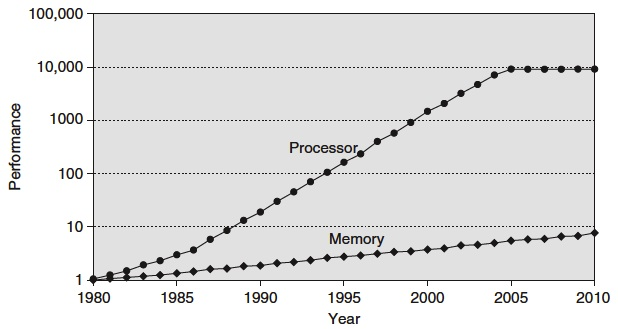
\includegraphics[width=3.5in]{graphics/CPUmemoryGap.jpg}
	\caption{Dette er ei tekning}
\end{figure}
\\
A prefetcher reduces this bottleneck by predicting which instructions are addressed next. Memory fetches are attempted to be done before the memory is needed by the microprocessor, leading to a decreased time where the processor is stuck in a waiting state. If the prefetched memory addresses differ from what was needed, the processor needs to access the RAM anyway. This is the worst case scenario, in which the cache has no effect on performance.

\section{Related Work}
The most basic prefetcher is called a sequential prefetcher. When a CPU is requesting a memory adress, the prefetcher will also fetch the next memory location. The performance of this prefetcher is very limtited since it does not have any form of heuristic. An improvement of this prefetcher is called tagged sequential prefetcher, which divides the sequences into blocks.

What these have in common, is that the prefetching is not based on statistics. They are instead deterministic fetches where a fixed group or single memory adress is fetched. To improve the performance, prefetching based on statistics were developed. These prefetchers will predict the next fetch statistically.   

A Reference Prediction Tables RPT is a prefetcher that is based on statistics. This type of prefetcher was first proposed in 1995 by Chan and Baer. A RPT contains a table with addresses of the missed fetches as index. Another variant of this is PC/DC prefetching. 

An another type of prefetching is called Delta Correlating Prediction, as described in \cite{reference:jahre}. Their purpose was to combine the delta correlating design of PC/DC and the storage efficiency of RPT. Compared to RC/DC, the DCPT reduces the complexity of the prefetching. This is done by recomputing the delta.

\section{Prefetcher Description}
The prefetcher has a pattern-seeking behaviour. It uses vectors to log observed fetch sequences, and ranks them based on how often the actual fetches correspond with the predicted sequences. This is achieved by logging combinations of three requests, thus making a link between two fetches and what we expect to be referenced after these. Every time the two requests are recognized, the third one is prefetched. If this is correct behaviour, the score of that particular sequence is raised. The next fetch is then always assumed to be the third fetch in the sequence that has been correct the most times.

The access sequences that occur the least frequent are more prone to being removed in favour of new sequences. This is done by continually raising a threshold. Sequences that are recognized and proven to be correct have their value increased. If entries fall under the threshold, they are removed when the cache is full and space is needed.



\section{Methodology}
\section*{Simulator}
The framework provided with the assignment was used for simulation. Our code was at first uploaded to the Kongull cluster, but this took a lot of time due to long queue times. The framework was therefore installed on one of our computers, running on Linux CentOS. This worked fine, but most of our other computers couldn't run the simulator because the GCC/G++ versions were too new. 

The simulator used was the modified M5 simulator provided with the assignment. 
\section{Results}


\begin{table}[!t]
\renewcommand{\arraystretch}{1.3}
\caption{Prefetcher results from the Kongull Cluster}
\label{table:results}
\centering
\begin{tabular}{|l|l|l|l|l|l|l|l|}
\hline
\bfseries Test & \bfseries Speedup & \bfseries IPC & \bfseries Accuracy & \bfseries Coverage & \bfseries Identified & \bfseries Issued\\
\hline
\hline
ammp 		& 0.999 & 0.082 & 0.060 & 0.000 & 13765492 & 32526\\
applu 		& 1.014 & 0.523 & 0.681 & 0.068 & 662896   & 233366\\
apsi 		& 1.015 & 1.507 & 0.628 & 0.020 & 60110    & 3777\\	
art110 		& 0.999 & 0.122 & 0.519 & 0.006 & 1728334  & 182419\\	
art470 		& 0.999 & 0.122 & 0.519 & 0.006 & 1728334  & 182419\\
bzip2\_graphic 	& 1.055 & 1.390 & 0.945 & 0.320 & 46207    & 31750\\
bzip2\_program 	& 1.021 & 1.515 & 0.962 & 0.128 & 10422    & 7394\\
bzip2\_source 	& 0.997 & 1.705 & 0.964 & 0.209 & 10327    & 7282\\
galgel 		& 0.998 & 0.443 & 0.388 & 0.008 & 249284   & 7166\\
swim 		& 0.978 & 0.669 & 0.309 & 0.019 & 2033005  & 144134\\
twolf 		& 0.997 & 0.423 & 0.632 & 0.001 & 1366 	   & 862	\\
wupwise 	& 1.059 & 0.791 & 0.343 & 0.187 & 279083   & 236426\\
\hline
\end{tabular}
\end{table}

As seen in table \ref{table:results}, the prefetcher does not provide a significant speedup. Some benchmarks provide better speedup than others, but the average speedup is only 1\%. There are some rather noteworthy variations regarding how the prefetcher performs on the different benchmarks, with some even reporting a decrease in speedup. These variations will be discussed further in the following section.

Some minor changes was also performed on the weighting in the scoring system, but the algorithm's speedup in the various tests remained relatively constant with negligible differences in the 0.1\% range.

The results in table \ref{table:results} adhere to the project guideline of keeping cache size under 8 Kb. Due to the strict limit this imposes on the prefetcher compared to the size of the address space, results from a run without these limits are included in table \ref{table:results2} for comparison.
As can be seen the results are fairly similar and provided an average speedup of 1.5\%. This is still low, but an increase from the implementation when the limit was imposed. As mentioned above, these results are only included for comparison.
Common and noteworthy for both of these results are that the prefetcher performs rather poor on the benchmarks that have long series of sequencial fetches. This will be further discussed in the next section.



\begin{table}[!t]
\renewcommand{\arraystretch}{1.3}
\caption{Prefetcher results without cache size limit}
\label{table:results2}
\centering
\begin{tabular}{|l|l|l|l|l|l|l|l|}
\hline
\bfseries Test & \bfseries Speedup & \bfseries IPC & \bfseries Accuracy & \bfseries Coverage & \bfseries Identified & \bfseries Issued\\
\hline
\hline
ammp 		& 1.000  &	0.082 &	0.210 &	0.001 &	13890679 &	51830\\
applu 		& 1.021 & 	0.527 &	0.606 &	0.111 &	1508604 & 	420247\\
apsi 		& 1.015 & 	1.508 &	0.680 &	0.052 &	70265 &	9120\\	
art110 		& 0.997 & 	0.122 &	0.607 &	0.033 &	13203897 &	981292\\	
art470 		& 0.997 & 	0.122 &	0.607 &	0.033 &	13203897 &	981292\\
bzip2\_graphic 	& 1.087 & 	1.431 &	0.915 &	0.356 &	52025 &	36610\\
bzip2\_program 	& 1.038 & 	1.540 &	0.771 &	0.197 &	17858 &	14172 	\\
bzip2\_source 	& 1.000 & 	1.709 &	0.768 &	0.259 &	14667 &	11336\\
galgel 		& 0.994 & 	0.442 &	0.432 &	0.028 &	310736 & 21353\\
swim 		& 0.978 & 	0.669 &	0.311 &	0.020 &	2125494 & 	149677\\
twolf 		& 1.003 & 	0.426 &	0.450 &	0.115 &	426956 & 	264981	\\
wupwise 	& 1.059 & 	0.791 &	0.343 &	0.187 &	279083 & 	236426\\
\hline
\end{tabular}
\end{table}



The dcpt algorithm originally proposed in \cite{reference:jahr} was also implemented and tested. For comparison the results are presented in table \ref{table:results3}. As can be seen from the table this implementation is conciderably faster on most benchmarks, and provided an overall avarage speedup of 5.5\%.

\begin{table}[!t]
\renewcommand{\arraystretch}{1.3}
\caption{DCPT Prefetcher results}
\label{table:results3}
\centering
\begin{tabular}{|l|l|l|l|l|l|l|l|}
\hline
\bfseries Test & \bfseries Speedup & \bfseries IPC & \bfseries Accuracy & \bfseries Coverage & \bfseries Identified & \bfseries Issued\\
\hline
\hline
ammp 		& 1.000 & 	0.082 &	0.148 &	0.000 &	13045 &	11424\\
applu 		& 1.074 & 	0.554 &	0.333 &	0.124 &	3424217 & 	831105\\
apsi 		& 1.084 & 	1.609 &	0.498 &	0.248 &	60278 &	59727\\	
art110 		& 1.056 & 	0.129 &	0.918 &	0.377 &	14786042 &	5651241\\	
art470 		& 1.056 & 	0.129 &	0.918 &	0.377 &	14786042 &	5651241\\
bzip2\_graphic 	& 1.090 & 	1.435 &	0.888 &	0.806 &	89642 &	85079 	\\
bzip2\_program 	& 1.059 & 	1.571 &	0.793 &	0.588 &	42511 &	41080 	\\
bzip2\_source 	& 0.992 & 	1.696 &	0.779 &	0.680 &	30397 &	29344\\
galgel 		& 1.013 & 	0.450 &	0.564 &	0.287 &	239107 &	 166359\\
swim 		& 1.046 & 	0.716 &	0.600 &	0.475 &	3102812 & 	1792901\\
twolf 		& 0.997 & 	0.423 &	0.380 &	0.002 &	6042 &	4990 		\\
wupwise 	& 1.240 & 	0.927 &	0.667 &	0.667 &	556492 & 	433877 	\\
\hline
\end{tabular}
\end{table}




% results from newer test
% result from dcpt
% results from Kaj

\section{Discussion}
The prefetcher did not result in any significant speed increase. It seemed like a good algorithm until it was tested. Seeing how many prefetches were done in each tests, it became obvious that attempting to log all patterns seen in such a big address space simply introduced complexity. There are extremely many address combinations, reducing the chance that the same patterns are visited multiple times. While the sequences probably will be visited again in the future, many others will take up a lot of the time, rendering the speedup negligible. The use of spatial and temporal locality therefore seems superior, both in terms of simplicity and result.

Table REFERER HER! shows an attempt to increase the speedup. It was thought that increasing the cache size would cause many more combinations to be stored, and thus avoid having sequences deleted before they were used due to the massive amount of possible sequences. The lack of speed increase shows that the algorithm was in the wrong from the beginning, and tries to predict too much. It assumes that things happen periodically, something there is no guarantee for in the benchmark tests.

%  Why no speed increase
% Attempts to increase speed. How and why
% Comment each test
% Compare with no-limit results
% Compare with DCPT
%
%
%

\section{Conclusion}
All in all the implentation of the prefetcher is comparable to an implementation based on the more probabilistic principle of locality. While the prefetcher detailed in this report attempts to map all of the the most frequent prefetch sequences and act based on these and only these, an approach based on the principle of locality would use much of the same concept, but would assume temporal and spatial correlations instead of writing a log based on observed prefetches. The idea of mapping possible sequences directly to their assumed following address might work in a predictable environment, but does not seem to function well in a more practical environment. 

Excluding the program counter from the algorithm in favor of more entries in the combinations pool proved to be a poor decision. The overall speedup dropped by approximately 4\% , and it can at least partially be linked directly to this choice. The added complexity also makes a clean, compact hardware implementation hard. 

Another reason for the prefetcher's low performance is the size of the accessed memory spaces. With so many combinations, it is not too likely that the same sequences will be frequented a lot. If the memory space was smaller, the same sequences might have been frequented more, resulting in higher accuracy. With the amount of addresses being high, the actual hits drown in the vast amount of possible sequences.

The project was a great learning experience, and has shown the importance of simulating ideas that sound like a good idea in theory. Writing the report was also a good practice in documenting the work, and even though the prefetcher provided a poor speedup, the project resulted in increased understanding of processors and their caches, in addition to document the impact the program counter has on prefetcher performance.





% if have a single appendix:
%\appendix[Proof of the Zonklar Equations]
% or
%\appendix  % for no appendix heading
% do not use \section anymore after \appendix, only \section*
% is possibly needed

% use appendices with more than one appendix
% then use \section to start each appendix
% you must declare a \section before using any
% \subsection or using \label (\appendices by itself
% starts a section numbered zero.)
%


\appendices
\section{Proof of the First Zonklar Equation}
Appendix one text goes here.

% you can choose not to have a title for an appendix
% if you want by leaving the argument blank
\section{}
Appendix two text goes here.


% use section* for acknowledgement
%\section*{Acknowledgment}


%The authors would like to thank...


% Can use something like this to put references on a page
% by themselves when using endfloat and the captionsoff option.
\ifCLASSOPTIONcaptionsoff
  \newpage
\fi



% trigger a \newpage just before the given reference
% number - used to balance the columns on the last page
% adjust value as needed - may need to be readjusted if
% the document is modified later
%\IEEEtriggeratref{8}
% The "triggered" command can be changed if desired:
%\IEEEtriggercmd{\enlargethispage{-5in}}

% references section

% can use a bibliography generated by BibTeX as a .bbl file
% BibTeX documentation can be easily obtained at:
% http://www.ctan.org/tex-archive/biblio/bibtex/contrib/doc/
% The IEEEtran BibTeX style support page is at:
% http://www.michaelshell.org/tex/ieeetran/bibtex/
%\bibliographystyle{IEEEtran}
% argument is your BibTeX string definitions and bibliography database(s)
%\bibliography{IEEEabrv,../bib/paper}
%
% <OR> manually copy in the resultant .bbl file
% set second argument of \begin to the number of references
% (used to reserve space for the reference number labels box)
\begin{thebibliography}{1}

\bibitem{reference:jahre} M.~Grannaes, M.~Jahre and L.~Natvig \emph{Storage Efficient Hardware Prefetching using Delta-Correlating Prediction Tables},
\hskip 1em plus 0.5em minus 0.4em\relax Journal of Instruction-Level Parallelism 13 (2011) 1-16

\bibitem{reference:opg} \emph{M5 simulator system TDT4260 Computer Architecture User documentation},
\hskip 1em plus 0.5em minus 0.4em\relax Assignment text

\bibitem{reference:spec} SPEC, "SPEC CPU2000 Benchmark Descriptions", 2007

\end{thebibliography}

% biography section
% 
% If you have an EPS/PDF photo (graphicx package needed) extra braces are
% needed around the contents of the optional argument to biography to prevent
% the LaTeX parser from getting confused when it sees the complicated
% \includegraphics command within an optional argument. (You could create
% your own custom macro containing the \includegraphics command to make things
% simpler here.)
%\begin{IEEEbiography}[{\includegraphics[width=1in,height=1.25in,clip,keepaspectratio]{mshell}}]{Michael Shell}
% or if you just want to reserve a space for a photo:

%\begin{IEEEbiography}{Michael Shell}
%Biography text here.
%\end{IEEEbiography}

% if you will not have a photo at all:
%\begin{IEEEbiographynophoto}{John Doe}
%Biography text here.
%\end{IEEEbiographynophoto}

% insert where needed to balance the two columns on the last page with
% biographies
%\newpage

%\begin{IEEEbiographynophoto}{Jane Doe}
%Biography text here.
%\end{IEEEbiographynophoto}

% You can push biographies down or up by placing
% a \vfill before or after them. The appropriate
% use of \vfill depends on what kind of text is
% on the last page and whether or not the columns
% are being equalized.

%\vfill

% Can be used to pull up biographies so that the bottom of the last one
% is flush with the other column.
%\enlargethispage{-5in}



% that's all folks
\end{document}
